Another track of research I have been following over the past years is the
learning of latent representations for time series.
These latent representations can either be mixture coefficients
(\emph{cf.} Sec.~\ref{sec:topics}) -- in which case time series are
represented as multinomial distributions over latent topics -- or intermediate
neural networks feature maps (as in Sec.~\ref{sec:cnn} and
Sec.~\ref{sec:early}) -- and then time series are represented through
filter activations they trigger.

More specifically, in Sec.~\ref{sec:early}, we focus on the task of early
classification of time series. In this context, a method is introduced.
This method
learns an intermediate representation from which both the decision of
triggering classification and the classification itself can be computed.


\section{Temporal Topic Models}
\label{sec:topics}

Topic models are mixture models that can deal with documents represented as
bags of features (BoF) and that can extract latent topics (a topic being a
distribution
over features) from a corpus of documents.
For these methods, time series are hence seen as bags of timestamped features.
In the methods presented here, the temporal dimension is either
included in the BoF representation (Sec.~\ref{sec:hdlsm}) or added in a
refinement step (Sec.~\ref{sec:oup}).

\subsection{Supervised Hierarchical Dirichlet Latent Semantic Motifs}
\label{sec:hdlsm}

In this work, we build upon the Hierarchical Dirichlet Latent Semantic Motifs
(HDLSM) topic model that was first introduced in~\cite{EmonetCVPR2011}.
This generative model relies on the extraction of motifs that encapsulate the
temporal information of the data.
It is able to automatically discover both the underlying number of motifs
needed to
model a given set of documents and the number and localization of motif
occurrences in each document, as shown in the Figure~\ref{fig:hdlsm}.

\begin{figure}
\centering
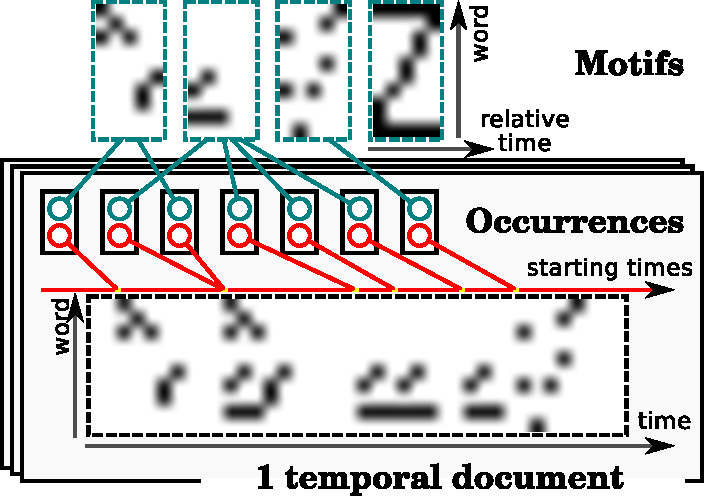
\includegraphics[width=.4\textwidth]{fig/hdlsm}
\caption{In the HDLSM model, a document is seen as a mixture of motif
occurrences. \label{fig:hdlsm}}
\end{figure}

The HDLSM model takes as input a set of quantized time series (aka temporal
documents).
More specifically, a time series is represented as a contingency table that
informs, for
each pair $(w, t)$, whether word (or a quantized feature) $w$ was
present in the time series at time index $t$ (in fact, it can also account for
the \emph{amount} of presence of word $w$ at time $t$).

HDLSM is a generative model. Its generative process can be described as
follows:
\begin{enumerate}
\item Generate a list of motifs, each motif $k$ being a 2D probability map
indicating how likely it is that word $w$ occurs at relative time $t_r$ after
the beginning of the motif.
\item For each document $j$, generate a list of occurrences, each occurrence having
a starting time $t_o$ and an associated motif $k$.
\item For each observation $i$ in document $j$:
  \begin{enumerate}
  \item Draw an occurrence from the list,
  \item Draw a pair $(w, t_r)$ from the associated motif,
  \item Generate the observation of word $w$ at time $t = t_o + t_r$.
  \end{enumerate}
\end{enumerate}

As stated above, motifs are represented as probabilistic maps.
Each map is drawn from a Dirichlet distribution.
This model makes intensive use of Dirichlet Processes (DP) to model the
possibly infinite number of motifs and occurrences.

To learn the parameters of the model, Gibbs sampling is used, in which it
is sufficient to re-sample motif assignments for both observations and
occurrences as well as occurrence starting times.
Other variables are either integrated out or deduced, when a deterministic
relation holds.

Our supervised variant relies on the same generative process except that an
extra component is added that maps motifs (denoted $z$)
to classes ($y$) in a supervised learning
context.
Therefore, this mapping needs to be learned and, once the model is trained,
classifying a new instance $\mathbf{x}$ consists in
(i) extracting motif probabilities $P(z | \mathbf{x})$ and
(ii) deriving class probabilities as:

\begin{equation}
    P(y | \mathbf{x}) = \sum_z P(y | z) P(z | \mathbf{x})
\end{equation}

We have used this model in the context of action recognition in
videos~\cite{tavenard:hal-00872048}.
Here, our \emph{words} are quantized spatio-temporal features and each time series
is the encoding of a video in which a single action is performed.
In this context, we show that our
model outperforms standard competitors that operate on the same quantized
features.

\subsection{Two-step Inference for Sequences of Ornstein Uhlenbeck Processes}
\label{sec:oup}

More recently, I have been involved in a project related to the surveillance of
the maritime traffic.
In this context, a major challenge
is the automatic identification of traffic flows from a set of observed
trajectories, in order to derive good management measures or to detect abnormal
or illegal behaviors for example.%
\footnote{This work was part of Pierre Gloaguen's postdoc.
This is joint work with Laetitia Chapel and Chloé Friguet.}

The model we have proposed in this context differs from the one described above
in several aspects:

\begin{itemize}
\item We are not in a supervised setting, we have no labelled data at our disposal
and our goal will rather be to extract meaningful trajectory clusters;
\item We are not looking for motifs to be localized in time series (with
a possible overlap between motifs, as in the method described above) but rather
in the segmentation of trajectories into homogeneous \emph{movement modes};
\item Each movement mode is described using a continuous time model;
\item In order to scale to larger datasets, stochastic variational inference is used
(in place of Gibbs sampling) for inference.
\end{itemize}

\subsubsection{Motivating Use Case}

The monitoring of maritime traffic relies on several sources of data, in a
rising context of maritime big data~\cite{garnier2016exploiting}.
Among these sources lies the Automatic Identification System (AIS), which
automatically collects messages from vessels around the world, at a high
frequency.
AIS data basically consist of GPS-like data, together with the instantaneous
speed and heading, and some vessel specific static information.
These data are characterized by their diversity as they (1) are collected at
different frequencies (2) have different lengths (3) are not necessarily
regularly sampled (4) represent very different behaviors, (5) share common
trends or similar subparts (\emph{movement modes}).

One major challenge in this context is the extraction of movement patterns
emerging from the observed data, considering trajectories that share similar
movement modes.
This issue can be restated from a machine learning point of view as a
large-scale clustering task.
This tasks involves the definition of clustering methods
that can handle such complex data while being efficient on large databases,
and that both cluster trajectories as a whole and detect common
sub-trajectories.

\subsubsection{Model}

We define a parametric framework to model trajectory data,
\emph{i.e.} sequences of geographical positions recorded through time.
The modeling framework aims to account for two levels of heterogeneity possibly
present in trajectory data:

\begin{enumerate}
\item heterogeneity of a vessel's movement within a single trajectory, and
\item heterogeneity between observed trajectories of several vessels.
\end{enumerate}

Following a common paradigm, we assume that a moving vessel's trajectory
is a heterogeneous sequence of patterns that we call \emph{movement modes}.
Different movement modes along a trajectory refer to different ways of moving
in terms of velocity distribution, reflecting different behaviors, activities,
or routes.
It is assumed that a given movement mode can be adopted by several vessels.

As done in~\cite{gurarie2017correlated}, we characterize
movement modes using a specific correlated velocity model, defined in a
continuous-time framework, namely the Ornstein-Uhlenbeck
Process~\cite{uhlenbeck1930theory} (OUP).
One important property of the OUP is that, under mild conditions,
the velocity process is an asymptotically stationary Gaussian Process, which
can be visualized in Figure~\ref{fig:oup}.

\begin{figure}
\centering
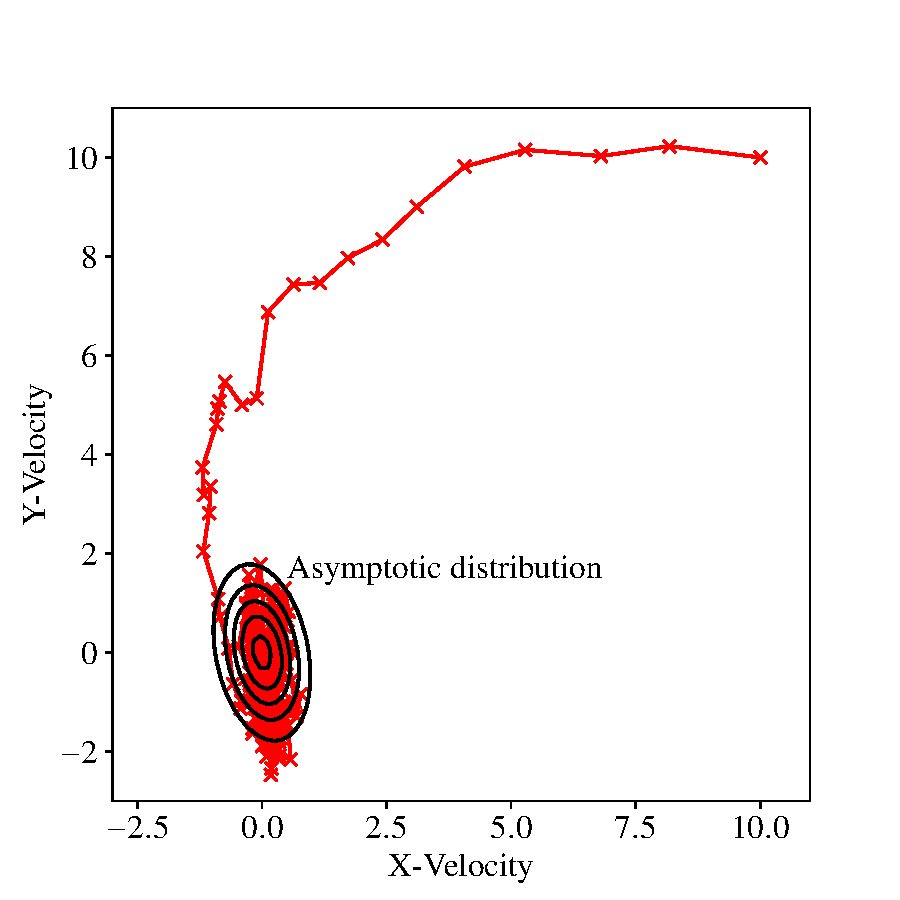
\includegraphics[width=.5\textwidth]{fig/oup}
\caption{Simulation of an OUP process. The starting point is in the
top-right corner and level sets of the asymptotic distribution are shown.
\label{fig:oup}}
\end{figure}

\subsubsection{Parameter estimation}

In order to perform scalable parameter inference and clustering of both
trajectories and GPS observations (into movement modes), we adopt a pragmatic
two step approach that takes advantage of the inherent properties of the OUP:

\begin{enumerate}
\item A first dual clustering is performed based on a simpler independent
Gaussian Mixture Model, in order to estimate potential movement modes and
trajectory clusters: it removes within mode autocorrelation in
the inference, and therefore facilitates the computations, yet it does not rely
on any temporal or sequential information.
Here again, we use a Hierarchical Dirichlet Process as a model for this
two-level clustering, hence allowing for infinite mixtures of both movement
modes and trajectory clusters.
The Gaussian hypothesis in this case is in line with our choice of the OUP as
our velocity process, since the OUP stationary distribution is Gaussian.
\item Among the estimated movement modes, only those meeting a temporal consistency
constraint are kept.
Parameters of these consistent movement modes are then estimated, and used to
reassign observations that were assigned to inconsistent movement modes (\emph{i.e.}
movement modes that do not last long enough to be considered reliable).
It ensures that only trajectory segments for which the stationary distribution
is reached are kept to estimate movement modes.
\end{enumerate}

The resulting consistent movement mode concept allows one to (1) have a good
estimation of OUP parameters within a movement mode (as a consistent sequence
will often be related to a large amount of points) and (2) filter out
"noise" movement modes gathering few observations in a temporally
inconsistent manner.

Parameter estimation for Step 1 described above is performed through stochastic
variational inference (SVI) to allow scalability to large datasets of AIS data,
and movement mode parameter estimation is performed using standard tools from
the OUP literature.

The clustering
step is predominant in the overall computational complexity at inference time,
since the OUP parameter estimation can be performed independently for each
movement mode.
It is quasilinear in the number of
observations and, as stochastic variational inference is used, parts of the
computations involved can easily be distributed.

\subsubsection{Results}

We have provided \href{https://github.com/rtavenar/ushant_ais}{a dataset} of
several
millions of observations in the AIS context.
This dataset is used in~\cite{gloaguen2020} to validate our model qualitatively
(through visual
analysis of extracted movement modes and trajectory clusters) and compare it to
a standard $k$-means clustering.
We intend to make this dataset a reference for future competitive methods to
compare on a
real-world large-scale trajectory dataset.

\section{Shapelet-based Representations and Convolutional Models}
\label{sec:cnn}

In this section, we will cover works that either relate to the Shapelet
representation for time series or to the family of (1D) Convolutional Neural
Networks, since these two families of methods are very similar in
spirit~\cite{lods:hal-01565207}.

\subsection{Data Augmentation for Time Series Classification}

We have shown in~\cite{leguennec:halshs-01357973} that augmenting time
series classification datasets was an efficient way to improve generalization
for Convolutional Neural Networks.
The data augmentation strategies that were investigated in this work are
local warping and window slicing and both lead to improvements.%
\footnote{This work was part of Arthur Le Guennec's Master internship.
We were co-supervising Arthur together with Simon Malinowski.}

\subsection{Learning to Mimic a Target Distance}
\label{sec:siamese}

Another track of research we have lead concerns unsupervised representation
learning for time series.
In this context, our approach has consisted in learning a representation in
order to mimic a target distance.%
\footnote{This work was part of Arnaud Lods' Master internship.
We were co-supervising Arnaud together with Simon Malinowski.}

As presented in Sec.~\ref{sec:dtw}, Dynamic Time Warping is a widely
used similarity measure for time series.
However, it suffers from its non differentiability and the fact that it does
not satisfy metric properties.
Our goal in~\cite{lods:hal-01565207} was to introduce a Shapelet model that
extracts latent representations such that Euclidean distance between latent
representations is as close as possible to Dynamic Time Warping between original
time series.
The resulting model is an instance of a Siamese Network, as illustrated in
Figure~\ref{fig:siamese}.

\begin{figure}[t]
\centering
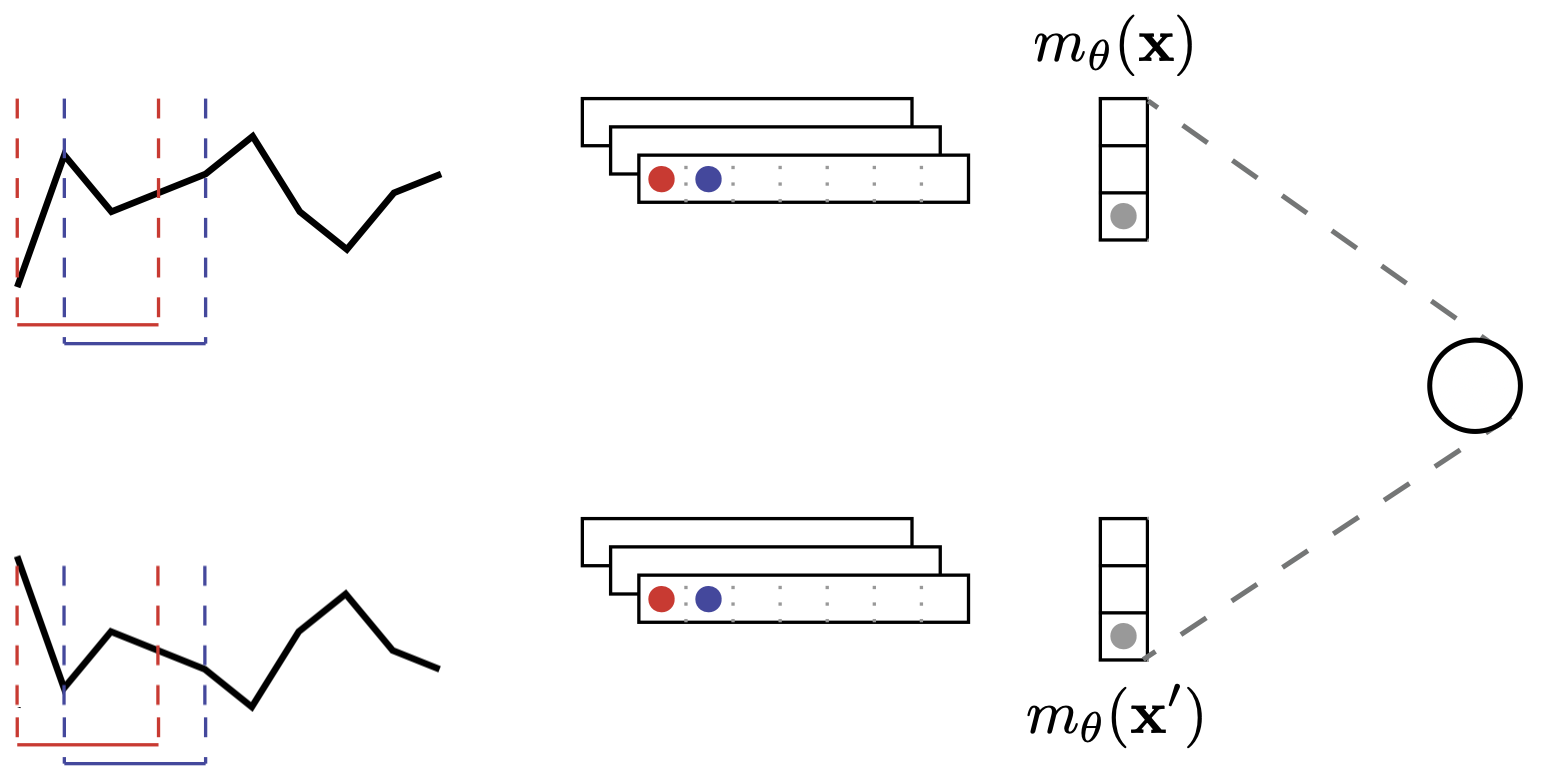
\includegraphics[width=.8\textwidth]{fig/siamese_ldps}
\caption{Shapelet extraction using a siamese network. \label{fig:siamese}}
\end{figure}

where $m_\theta(\cdot)$ is the feature extraction part of the model that
maps a time series to its shapelet transform representation.

We have shown that such a model could be used as a feature extractor on top of
which a $k$-means clustering could operate efficiently.
We have also shown in~\cite{carlinisperandio:hal-01841995} that this
representation is useful for time series indexing tasks.

\subsection{Including Localization Information}

The shapelet transform, as defined above, does not hold localization
information. Several options could be considered to add such kind of
information. First, the global pooling step could be turned into local pooling
to keep track of local shapelet distances.
In~\cite{guilleme:hal-02513295}, we rather focused on augmenting the feature
representation with shapelet match localization features.%
\footnote{This work was part of Mael Guillemé's PhD thesis.
I was not involved in Mael's PhD supervision.}

Relying on a set of random shapelets (shapelets that are extracted uniformly at
random from the set of all subseries in the training set)
$\{\mathbf{s_k}\}_{k < p}$,
each time series is embedded into a $2p$-dimensional feature that stores, for
each shapelet, the shapelet distance $d_{\mathbf{s_k}}(\cdot)$ as well as
optimal  match localization $l_{\mathbf{s_k}}(\cdot)$:

\begin{eqnarray}
    d_{\mathbf{s_k}}(\mathbf{x}) &=& \min_t
        \|\mathbf{x}_{t \rightarrow t+L_k} - \mathbf{s_k}\| \\
    l_{\mathbf{s_k}}(\mathbf{x}) &=& \arg \min_t
        \|\mathbf{x}_{t \rightarrow t+L_k} - \mathbf{s_k}\|
\end{eqnarray}

where $L_k$ is the length of the $k$-th shapelet and
$\mathbf{x}_{t \rightarrow t+L_k}$
is the subseries from $\mathbf{x}$ that starts at timestamp $t$ and has length
$L_k$.

In the random shapelet setting, a large number of shapelets are drawn and
feature selection is used afterwards to focus on most useful shapelets.
In our specific context, we have introduced a structured feature selection
mechanism that allows, for each shapelet, to either:

\begin{itemize}
\item discard all information (match magnitude and localization);
\item keep shapelet distance information and discard localization information;
\item keep all information (match magnitude and localization).
\end{itemize}

To do so, we have introduced a modified Group-Lasso (called
Semi-Sparse Group Lasso) loss that allows to enforce sparsity on some individual
variables only:

\begin{equation}
    \mathcal{L}^{\mathrm{SSGL}}(\mathbf{x}, y, \boldsymbol{\theta}) =
        \mathcal{L}(\mathbf{x}, y, \boldsymbol{\theta})
        + \alpha \lambda
            \left\| \mathbf{M}_\text{ind} \boldsymbol{\beta} \right\|_1
        + (1-\alpha) \lambda \sum_{k=1}^{K} \sqrt{p_k}
            \left\| \boldsymbol{\beta}^{(k)} \right\|_2
\end{equation}

where $\mathbf{M}_\text{ind}$ is a diagonal indicator matrix that has ones on
the diagonal for features that could be discarded individually (localization
features in our random shapelet case), $\boldsymbol{\theta}$ is the set of
all model weights, including weights $\boldsymbol{\beta}$ that are directly
connected to the features (\emph{ie.} these are weights from the first layer), that
are organized in groups $\boldsymbol{\beta}^{(k)}$ of size $p_k$ ($p_k=2$ in the
random shapelet context, each group corresponding to a different shapelet).

Figure~\ref{fig:ssgl} illustrates the benefit of our SSGL regularization scheme
when groups of variables exist in the data and semi-sparse hypothesis holds.

\begin{figure}[t]
\centering
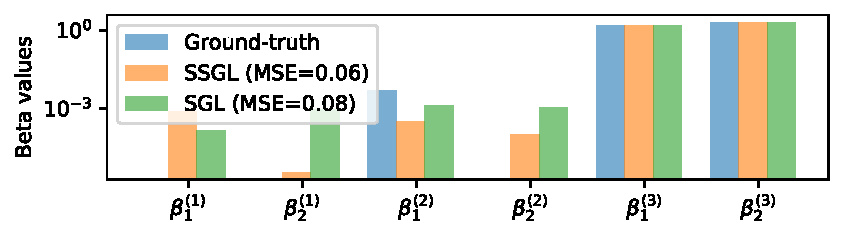
\includegraphics[width=.8\textwidth]{fig/ssgl}
\caption{Semi-Sparse Group Lasso regularization. Coefficients learned using
different regularization schemes for a linear regression problem. Ground-truth
coefficients are reported in blue.\label{fig:ssgl}}
\end{figure}

and one can notice that SSGL slightly outperforms Sparse-Group Lasso (SGL) in
terms of both Mean Squared Error (MSE) and estimation of zero coefficients.

When applied to the specific case of random shapelets, we have shown that this
lead to improved accuracy as soon as datasets are large enough for coefficients
to be estimated properly.

\subsection{Learning Shapelets that Look Like Time Series Snippets}

Early works on shapelet-based time series classification relied on a direct
extraction of shapelets as time series snippets from the training set.
Selected shapelets could be used \emph{a posteriori} to explain the classifier's
decision from realistic features.
However, the shapelet enumeration and selection processes were either very
costly or the selection was fast but did not yield good performance.
Jointly learning a shapelet-based representation of the series in the dataset
and classifying the series according to this
representation~\cite{grabocka2014learning} allowed to obtain
discriminative shapelets in a much more efficient way.%
\footnote{This work is part of Yichang Wang's PhD thesis.
I am co-supervising Yichang with Élisa Fromont, Rémi Emonet and Simon
Malinowski.}

However, if the learned shapelets are definitively discriminative, they are
often very different from actual pieces of a real series in the
dataset. As such, these shapelets might not be suited to explain a particular
classifier's decision.
In~\cite{wang2020},
we rely on a simple convolutional network to classify time
series and use an adversarial network that acts as a regularizer to ensure that
learned shapelets are un-distinguishable from actual time series pieces from
the training set.

\section{Early Classification of Time Series}
\label{sec:early}

Early classification of time series is the task of performing a classification
as early as possible for an incoming time series.
% Because of the specificity of this task, I will use in this section the
% notation $\mathbf{x}_{\rightarrow t}$ to denote the time series $\mathbf{x}$
% truncated after $t$ timestamps.

I have worked on two methods for this task.
The first one is a slight improvement
over~\cite{dachraoui2015early} and the second one relies on a
representation-learning strategy.

\subsection{Optimizing a Composite Loss for Early Classification}

\cite{dachraoui2015early} introduces a composite loss function for early
classification of time series that balances earliness and accuracy.

The cost function is of the following form:

\begin{equation}
\mathcal{L}(\mathbf{x}_{\rightarrow t}, y, t, \boldsymbol{\theta}) =
    \mathcal{L}_c(\mathbf{x}_{\rightarrow t}, y, \boldsymbol{\theta}) + \alpha t
\label{eq:loss_early}
\end{equation}

\noindent
where $\mathcal{L}_c(\cdot,\cdot,\cdot)$ is a
classification loss and $t$ is the time at which a
decision is triggered by the system.
In this setting, $\alpha$ drives the tradeoff between accuracy and earliness
and is supposed to be a hyper-parameter of the method.

The authors rely on (i) a clustering of the
training
time series and (ii) individual classifiers $m_t(\cdot)$ trained at all possible
timestamps, so as to be able to predict, at time $t$, an expected cost for all
times $t + \tau$ with $\tau \geq 0$:

\begin{equation}
    f_\tau(\mathbf{x}_{\rightarrow t}, y) =
        \sum_k \left[ P(C_k | \mathbf{x}_{\rightarrow t})
        \sum_i \left( P(y=i | C_k)
        \left( \sum_{j \neq i} P_{t+\tau}(\hat{y} = j | y=i, C_k)
        \right) \right)
        \right]
        + \alpha t
        \label{eq:dachraoui}
\end{equation}

where:

\begin{itemize}
\item $P(C_k | \mathbf{x}_{\rightarrow t})$ is a soft-assignment weight of
$\mathbf{x}_{\rightarrow t}$ to cluster $C_k$;
\item $P(y=i | C_k)$ is obtained from a contingency table that stores the number of
training time series of each class in each cluster;
\item $P_{t+\tau}(\hat{y} = j | y=i, C_k)$ is obtained through training time
confusion matrices built on time series from cluster $C_k$ using classifier
$m_{t+\tau}(\cdot)$.
\end{itemize}

At test time, if a series is observed up to time $t$ and if, for all positive
$\tau$ we have
$f_\tau(\mathbf{x}_{\rightarrow t}, y) \geq f_0(\mathbf{x}_{\rightarrow t}, y)$,
then a decision is made using classifier $m_t(\cdot)$.

\subsubsection{Limitations of the Clustering}

Relying on Equation \eqref{eq:dachraoui} to decide prediction time can be
tricky. We show in the following that in some cases (related to specific
configurations of the training time confusion matrices), such an approach will
lead to undesirable behaviors.%
\footnote{This unpublished note is part of François Painblanc's PhD work.
We are co-supervising François together with Laetitia Chapel and Chloé Friguet.}

Using Bayes' rule, Equation \eqref{eq:dachraoui} can be re-written

\begin{eqnarray}
    f_\tau(\mathbf{x}_{\rightarrow t}, y) &=&
        \sum_k P(C_k | \mathbf{x}_{\rightarrow t})
        \sum_i
        \sum_{j \neq i} P_{t+\tau}(\hat{y} = j, y=i | C_k)
        + \alpha t \\
    &=&
        \sum_k P(C_k | \mathbf{x}_{\rightarrow t})
        \underbrace{\sum_i 1 - P_{t+\tau}(\hat{y} = i, y=i | C_k)}_{A_{t+\tau}(C_k)}
        + \alpha t \\
\end{eqnarray}

where $A_{t+\tau}(C_k)$ is the sum of off-diagonal elements in the (normalized)
training time confusion matrix built from time series in cluster $k$ using
classifier $m_{t+\tau}(\cdot)$.

In practice, this means that if the sum of off-diagonal elements of confusion
matrices is equal to the same $A_{t+\tau}$ for all clusters, then this method
will make a decision on the most adequate prediction time without taking the
data $\mathbf{x}_{\rightarrow t}$ into account:

\begin{eqnarray}
    f_\tau(\mathbf{x}_{\rightarrow t}, y) &=&
        \sum_k P(C_k | \mathbf{x}_{\rightarrow t})
        A_{t+\tau}
        + \alpha t \\
     &=&
        A_{t+\tau} + \alpha t \\
\end{eqnarray}

In other words, for this method to adapt the decision time $t$ in a
data-dependent fashion, it is important that accuracy differs
significantly between clusters, which is a condition that is difficult to ensure
\emph{a priori}.

\subsection{Pushing the Method to the Limit Case}

In~\cite{tavenard:halshs-01339007}, we pushed this method to its limit case
where the number of clusters is equal to the number of training time series.
In this case, the limitation exposed above does not hold anymore.

We showed superior loss optimization capabilities with this approach, at the
cost of a larger computational complexity.

We also showed that in order to limit inference time complexity, one could
learn a \emph{decision triggering classifier} that, based on the time series
$\mathbf{x}_{\rightarrow t}$, predicts whether a decision should be triggered
or not.
In this setting, the target values $\gamma_t$ used to train this
\emph{decision triggering classifier}
were computed from expected costs $f_\tau$ presented above:

\begin{equation}
    \gamma_t(\mathbf{x}_{\rightarrow t}, y) = \left\{
        \begin{array}{l}
            1 \text{ if } f_{0}(\mathbf{x}_{\rightarrow t}, y) =
                \min_{\tau \geq 0} f_{\tau}(\mathbf{x}_{\rightarrow t}, y) \\
            0 \text{ otherwise. }
        \end{array} \right.
\end{equation}

In other words, decision making is here seen as a two-step process where a
first classifier (\emph{decision triggering classifier}) decides whether a decision
should be made, in which case a
second classifier is used to determine the class to be predicted (the latter
classifier is $m_t(\cdot)$, the same as for other methods).

\subsection{Representation Learning for Early Classification}

The previous approach has several shortcomings.
First, it requires to learn a classifier $m_t(\cdot)$ for each possible time
series length $t$, which is very costly.
Second, both classifiers (the one that decides whether a decision should be
made, and the one that actually makes the decision) are seen as independent
models, while they are, in practice, closely related.
Finally, the loss function presented in Equation \eqref{eq:loss_early} requires
a careful choice of hyper-parameter $\alpha$ that might not be easy to
determine in
practice.%
\footnote{This work is part of Marc Rußwurm's PhD work.
Marc is a PhD student from TU Munich who came to France for a
4-month period in 2018-2019. I was co-supervising Marc with Nicolas Courty
and Sébastien Lefèvre during his stay.}

We have hence proposed a representation learning framework that
addresses these three limitations~\cite{ruwurm:hal-02174314}.

In more detail, we rely on a feature extraction module (that can either be
made of causal convolutions or recurrent submodules) to extract a fixed-sized
representation $h_t$ from an incoming time series $\mathbf{x}_{\rightarrow t}$.
An important point here is that this feature extractor should operate on time
series whatever their length (and hence a different feature extractor need not
to be learned for each time series length).
Then, this feature is provided as input to two different heads, as shown in
Figure~\ref{fig:early}.

\begin{figure}[t]
\centering
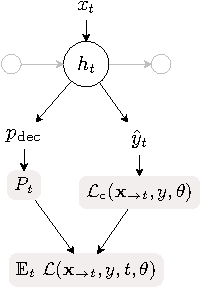
\includegraphics[width=.3\textwidth]{fig/early_module_cropped}
\caption{End-to-end differentiable early classification model.
Grey cells correspond to quantities that are
computed from the model outputs. \label{fig:early}}
\end{figure}

\begin{itemize}
\item The first head (left) outputs a probability $p_\text{dec}$ of making a
decision at
time $t$ given that no decision has been made before: it plays the same role
as the \emph{decision triggering classifier} presented above and from the series of
$p_\text{dec}$ values, one can compute the probability $P_t$ of making a
decision at time $t$;
\item The second head is the standard classification head that effectively produces
a classification if the first head triggered it.
\end{itemize}

Hence, provided that we have a differentiable early classification loss
function, we are able to learn all parameters of this model end-to-end.
Our last contribution in this context is the design of a loss function that
does not lead to dumb optimal solutions (\emph{e.g.}, trigger all
classifications at
the first time stamp, whatever the data).
We introduced the following loss function:

\begin{equation}
    \mathcal{L}(\mathbf{x}_{\rightarrow t}, y, t, \boldsymbol{\theta}) =
        \alpha \mathcal{L}_c(\mathbf{x}_{\rightarrow t}, y, \boldsymbol{\theta})
            - (1-\alpha) P_{\boldsymbol{\theta}}(m_t(\mathbf{x}_{\rightarrow t})=y)
            \left( \frac{T-t}{T} \right)
\end{equation}

\noindent
where $P_{\boldsymbol{\theta}}(m_t(\mathbf{x}_{\rightarrow t})=y)$ is the
probability (as
assigned by the classification model) to generate $y$ as an output and $T$ is
the total length of the time series (\emph{i.e.} the maximum timestamp at which
a decision can be made).
The second part in this loss function is an earliness reward, which is taken
into account iff the provided decision is sound (\emph{i.e.} the correct class
is
predicted with non-zero probability).
When the decision time is drawn from the
multinomial distribution of parameters $\{P_t\}_{t \in [0, T-1]}$, the overall
loss is now:
\begin{equation}
    \mathbb{E}_{t \sim \mathcal{M}(P_0, \dots , P_{T-1})}
        \mathcal{L}(\mathbf{x}_{\rightarrow t}, y, t, \boldsymbol{\theta})
\end{equation}
and gradients can be back-propagated through both heads of the model, hence
allowing to jointly learn the early decision mechanism and the predictor.

We have shown that this model outperforms all known baselines in terms of both
time complexity and earliness/accuracy tradeoff, especially for large scale
datasets.
Moreover, we have presented an application of this model to the monitoring of
agriculture, and demonstrated its ability to trigger class-specific early
decisions in this context in~\cite{ruwurm:hal-02343851}.

